\documentclass[]{article}
\usepackage{lmodern}
\usepackage{amssymb,amsmath}
\usepackage{ifxetex,ifluatex}
\usepackage{fixltx2e} % provides \textsubscript
\ifnum 0\ifxetex 1\fi\ifluatex 1\fi=0 % if pdftex
  \usepackage[T1]{fontenc}
  \usepackage[utf8]{inputenc}
\else % if luatex or xelatex
  \ifxetex
    \usepackage{mathspec}
  \else
    \usepackage{fontspec}
  \fi
  \defaultfontfeatures{Ligatures=TeX,Scale=MatchLowercase}
\fi
% use upquote if available, for straight quotes in verbatim environments
\IfFileExists{upquote.sty}{\usepackage{upquote}}{}
% use microtype if available
\IfFileExists{microtype.sty}{%
\usepackage{microtype}
\UseMicrotypeSet[protrusion]{basicmath} % disable protrusion for tt fonts
}{}
\usepackage[margin=1in]{geometry}
\usepackage{hyperref}
\hypersetup{unicode=true,
            pdftitle={HW04},
            pdfborder={0 0 0},
            breaklinks=true}
\urlstyle{same}  % don't use monospace font for urls
\usepackage{color}
\usepackage{fancyvrb}
\newcommand{\VerbBar}{|}
\newcommand{\VERB}{\Verb[commandchars=\\\{\}]}
\DefineVerbatimEnvironment{Highlighting}{Verbatim}{commandchars=\\\{\}}
% Add ',fontsize=\small' for more characters per line
\usepackage{framed}
\definecolor{shadecolor}{RGB}{248,248,248}
\newenvironment{Shaded}{\begin{snugshade}}{\end{snugshade}}
\newcommand{\KeywordTok}[1]{\textcolor[rgb]{0.13,0.29,0.53}{\textbf{#1}}}
\newcommand{\DataTypeTok}[1]{\textcolor[rgb]{0.13,0.29,0.53}{#1}}
\newcommand{\DecValTok}[1]{\textcolor[rgb]{0.00,0.00,0.81}{#1}}
\newcommand{\BaseNTok}[1]{\textcolor[rgb]{0.00,0.00,0.81}{#1}}
\newcommand{\FloatTok}[1]{\textcolor[rgb]{0.00,0.00,0.81}{#1}}
\newcommand{\ConstantTok}[1]{\textcolor[rgb]{0.00,0.00,0.00}{#1}}
\newcommand{\CharTok}[1]{\textcolor[rgb]{0.31,0.60,0.02}{#1}}
\newcommand{\SpecialCharTok}[1]{\textcolor[rgb]{0.00,0.00,0.00}{#1}}
\newcommand{\StringTok}[1]{\textcolor[rgb]{0.31,0.60,0.02}{#1}}
\newcommand{\VerbatimStringTok}[1]{\textcolor[rgb]{0.31,0.60,0.02}{#1}}
\newcommand{\SpecialStringTok}[1]{\textcolor[rgb]{0.31,0.60,0.02}{#1}}
\newcommand{\ImportTok}[1]{#1}
\newcommand{\CommentTok}[1]{\textcolor[rgb]{0.56,0.35,0.01}{\textit{#1}}}
\newcommand{\DocumentationTok}[1]{\textcolor[rgb]{0.56,0.35,0.01}{\textbf{\textit{#1}}}}
\newcommand{\AnnotationTok}[1]{\textcolor[rgb]{0.56,0.35,0.01}{\textbf{\textit{#1}}}}
\newcommand{\CommentVarTok}[1]{\textcolor[rgb]{0.56,0.35,0.01}{\textbf{\textit{#1}}}}
\newcommand{\OtherTok}[1]{\textcolor[rgb]{0.56,0.35,0.01}{#1}}
\newcommand{\FunctionTok}[1]{\textcolor[rgb]{0.00,0.00,0.00}{#1}}
\newcommand{\VariableTok}[1]{\textcolor[rgb]{0.00,0.00,0.00}{#1}}
\newcommand{\ControlFlowTok}[1]{\textcolor[rgb]{0.13,0.29,0.53}{\textbf{#1}}}
\newcommand{\OperatorTok}[1]{\textcolor[rgb]{0.81,0.36,0.00}{\textbf{#1}}}
\newcommand{\BuiltInTok}[1]{#1}
\newcommand{\ExtensionTok}[1]{#1}
\newcommand{\PreprocessorTok}[1]{\textcolor[rgb]{0.56,0.35,0.01}{\textit{#1}}}
\newcommand{\AttributeTok}[1]{\textcolor[rgb]{0.77,0.63,0.00}{#1}}
\newcommand{\RegionMarkerTok}[1]{#1}
\newcommand{\InformationTok}[1]{\textcolor[rgb]{0.56,0.35,0.01}{\textbf{\textit{#1}}}}
\newcommand{\WarningTok}[1]{\textcolor[rgb]{0.56,0.35,0.01}{\textbf{\textit{#1}}}}
\newcommand{\AlertTok}[1]{\textcolor[rgb]{0.94,0.16,0.16}{#1}}
\newcommand{\ErrorTok}[1]{\textcolor[rgb]{0.64,0.00,0.00}{\textbf{#1}}}
\newcommand{\NormalTok}[1]{#1}
\usepackage{graphicx,grffile}
\makeatletter
\def\maxwidth{\ifdim\Gin@nat@width>\linewidth\linewidth\else\Gin@nat@width\fi}
\def\maxheight{\ifdim\Gin@nat@height>\textheight\textheight\else\Gin@nat@height\fi}
\makeatother
% Scale images if necessary, so that they will not overflow the page
% margins by default, and it is still possible to overwrite the defaults
% using explicit options in \includegraphics[width, height, ...]{}
\setkeys{Gin}{width=\maxwidth,height=\maxheight,keepaspectratio}
\IfFileExists{parskip.sty}{%
\usepackage{parskip}
}{% else
\setlength{\parindent}{0pt}
\setlength{\parskip}{6pt plus 2pt minus 1pt}
}
\setlength{\emergencystretch}{3em}  % prevent overfull lines
\providecommand{\tightlist}{%
  \setlength{\itemsep}{0pt}\setlength{\parskip}{0pt}}
\setcounter{secnumdepth}{0}
% Redefines (sub)paragraphs to behave more like sections
\ifx\paragraph\undefined\else
\let\oldparagraph\paragraph
\renewcommand{\paragraph}[1]{\oldparagraph{#1}\mbox{}}
\fi
\ifx\subparagraph\undefined\else
\let\oldsubparagraph\subparagraph
\renewcommand{\subparagraph}[1]{\oldsubparagraph{#1}\mbox{}}
\fi

%%% Use protect on footnotes to avoid problems with footnotes in titles
\let\rmarkdownfootnote\footnote%
\def\footnote{\protect\rmarkdownfootnote}

%%% Change title format to be more compact
\usepackage{titling}

% Create subtitle command for use in maketitle
\providecommand{\subtitle}[1]{
  \posttitle{
    \begin{center}\large#1\end{center}
    }
}

\setlength{\droptitle}{-2em}

  \title{HW04}
    \pretitle{\vspace{\droptitle}\centering\huge}
  \posttitle{\par}
    \author{}
    \preauthor{}\postauthor{}
    \date{}
    \predate{}\postdate{}
  

\begin{document}
\maketitle

\begin{Shaded}
\begin{Highlighting}[]
\KeywordTok{library}\NormalTok{(tidyr)}
\KeywordTok{library}\NormalTok{(tidyverse)}
\end{Highlighting}
\end{Shaded}

\begin{verbatim}
## -- Attaching packages ------------------------------------------------------------------------------------- tidyverse 1.2.1 --
\end{verbatim}

\begin{verbatim}
## v ggplot2 3.2.0     v purrr   0.3.2
## v tibble  2.1.3     v dplyr   0.8.3
## v readr   1.3.1     v stringr 1.4.0
## v ggplot2 3.2.0     v forcats 0.4.0
\end{verbatim}

\begin{verbatim}
## Warning: package 'ggplot2' was built under R version 3.5.2
\end{verbatim}

\begin{verbatim}
## Warning: package 'tibble' was built under R version 3.5.2
\end{verbatim}

\begin{verbatim}
## Warning: package 'purrr' was built under R version 3.5.2
\end{verbatim}

\begin{verbatim}
## Warning: package 'dplyr' was built under R version 3.5.2
\end{verbatim}

\begin{verbatim}
## Warning: package 'stringr' was built under R version 3.5.2
\end{verbatim}

\begin{verbatim}
## Warning: package 'forcats' was built under R version 3.5.2
\end{verbatim}

\begin{verbatim}
## -- Conflicts ---------------------------------------------------------------------------------------- tidyverse_conflicts() --
## x dplyr::filter() masks stats::filter()
## x dplyr::lag()    masks stats::lag()
\end{verbatim}

\begin{Shaded}
\begin{Highlighting}[]
\KeywordTok{library}\NormalTok{(gapminder)}
\end{Highlighting}
\end{Shaded}

1.1

Installed tidyverse again so that I could get the pivot functions. I
selected the columns that mattered to me, and then I filtered so that
the countries that I would focus on were Canada and Albania.

Then I left the year the same, but changed the columns to represent
Canada and Albania, and had life expectancy values under those

I could not figure out how to Change the names to ``Life Expectancy
Canada'' and ``Life Expectancy Albania''

\begin{Shaded}
\begin{Highlighting}[]
\KeywordTok{print}\NormalTok{(}
\NormalTok{gapminderlife<-gapminder}\OperatorTok
\StringTok{  }\KeywordTok{select}\NormalTok{(year,country,lifeExp)}\OperatorTok
\StringTok{  }\NormalTok{dplyr}\OperatorTok{::}\KeywordTok{filter}\NormalTok{(country}\OperatorTok{==}\StringTok{"Canada"}\OperatorTok{|}\NormalTok{country}\OperatorTok{==}\StringTok{"Albania"}\NormalTok{)}\OperatorTok\StringTok{ }
\StringTok{  }\KeywordTok{pivot_wider}\NormalTok{(}\DataTypeTok{id_cols     =} \KeywordTok{c}\NormalTok{(}\OperatorTok{-}\NormalTok{country,}\OperatorTok{-}\NormalTok{lifeExp),}
              \DataTypeTok{names_from  =}\NormalTok{ country, }
              \DataTypeTok{values_from =}\NormalTok{ lifeExp)}
\NormalTok{)}
\end{Highlighting}
\end{Shaded}

\begin{verbatim}
## # A tibble: 12 x 3
##     year Albania Canada
##    <int>   <dbl>  <dbl>
##  1  1952    55.2   68.8
##  2  1957    59.3   70.0
##  3  1962    64.8   71.3
##  4  1967    66.2   72.1
##  5  1972    67.7   72.9
##  6  1977    68.9   74.2
##  7  1982    70.4   75.8
##  8  1987    72     76.9
##  9  1992    71.6   78.0
## 10  1997    73.0   78.6
## 11  2002    75.7   79.8
## 12  2007    76.4   80.7
\end{verbatim}

\begin{Shaded}
\begin{Highlighting}[]
\CommentTok{#1.2 I plotted the countries against each other using geom_point for a scatterplot.}

\NormalTok{gapminderlife }\OperatorTok\StringTok{ }
\StringTok{  }\KeywordTok{ggplot}\NormalTok{(}\KeywordTok{aes}\NormalTok{(}\DataTypeTok{x =}\NormalTok{ Canada, }\DataTypeTok{y =}\NormalTok{ Albania)) }\OperatorTok{+}\StringTok{ }
\StringTok{  }\KeywordTok{geom_point}\NormalTok{() }\OperatorTok{+}\StringTok{ }\CommentTok{# }
\StringTok{    }\KeywordTok{labs}\NormalTok{(}
      \DataTypeTok{x=}\StringTok{"Canada Life Expectancy in years"}\NormalTok{,}
      \DataTypeTok{y=}\StringTok{"Albania Life Expectancy in years"}\NormalTok{,}
      \DataTypeTok{title =} \StringTok{"Life Expectancy of Canada vs Albania"}\NormalTok{,}
      \DataTypeTok{subtitle =} \StringTok{"taken from Gapminder data"}
\NormalTok{      ) }
\end{Highlighting}
\end{Shaded}

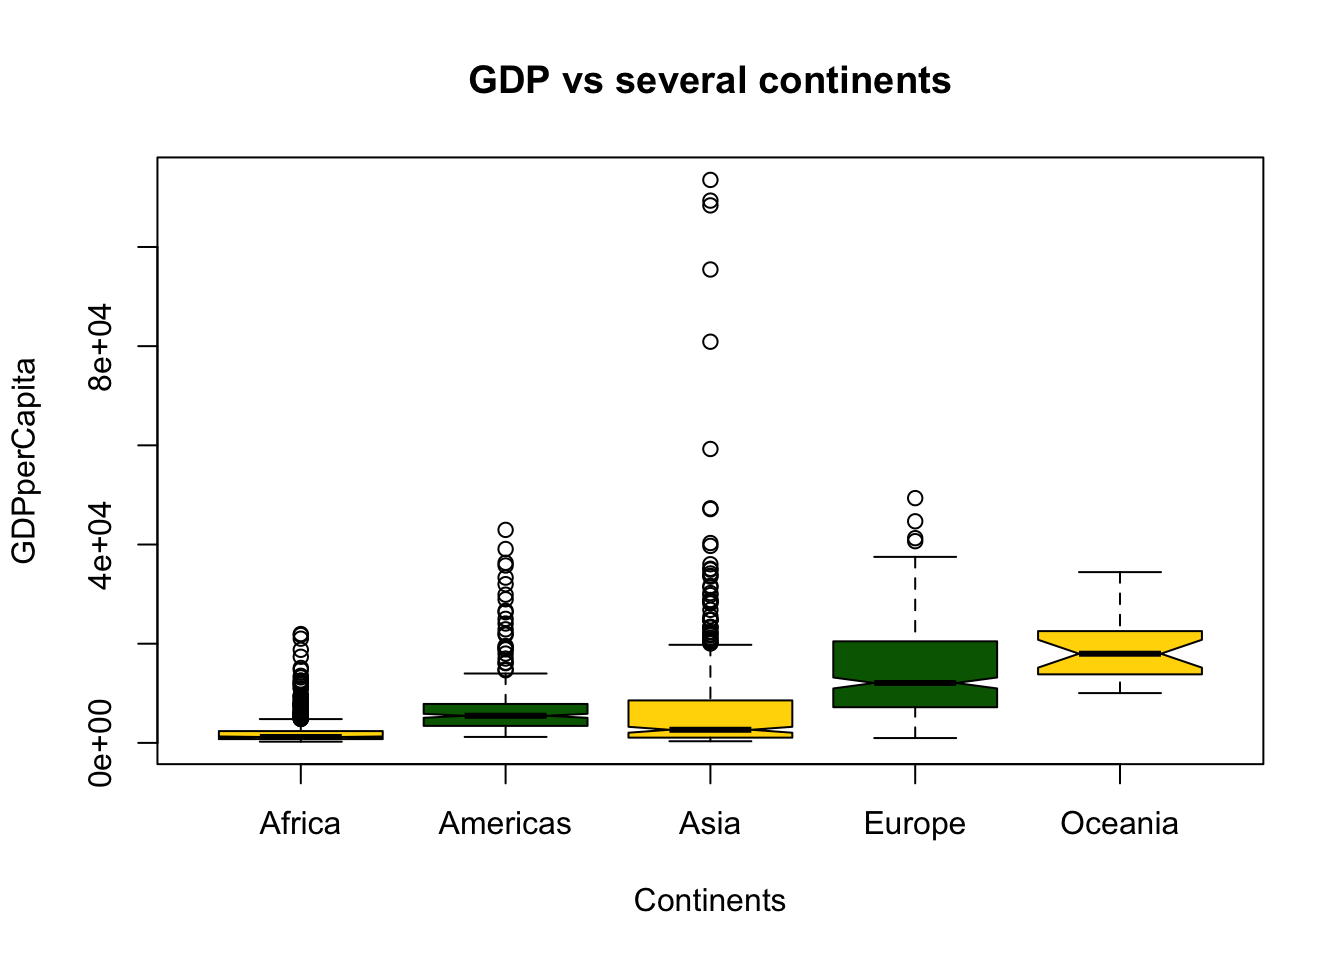
\includegraphics{HW04_files/figure-latex/unnamed-chunk-2-1.pdf}

\begin{Shaded}
\begin{Highlighting}[]
\CommentTok{#Then I returned the data to an original state, with year staying the same, and country and life expectancy going into the long format}

\NormalTok{print}
\end{Highlighting}
\end{Shaded}

\begin{verbatim}
## function (x, ...) 
## UseMethod("print")
## <bytecode: 0x7fb0ec111e40>
## <environment: namespace:base>
\end{verbatim}

\begin{Shaded}
\begin{Highlighting}[]
\NormalTok{(gapminderlifelong<-gapminderlife }\OperatorTok\StringTok{ }
\StringTok{  }\KeywordTok{pivot_longer}\NormalTok{(}\DataTypeTok{cols     =}\NormalTok{ (}\OperatorTok{-}\NormalTok{year),}
              \DataTypeTok{names_to  =} \StringTok{"country"}\NormalTok{, }
              \DataTypeTok{values_to =} \StringTok{"lifeExp"}\NormalTok{) }
\NormalTok{)}
\end{Highlighting}
\end{Shaded}

\begin{verbatim}
## # A tibble: 24 x 3
##     year country lifeExp
##    <int> <chr>     <dbl>
##  1  1952 Albania    55.2
##  2  1952 Canada     68.8
##  3  1957 Albania    59.3
##  4  1957 Canada     70.0
##  5  1962 Albania    64.8
##  6  1962 Canada     71.3
##  7  1967 Albania    66.2
##  8  1967 Canada     72.1
##  9  1972 Albania    67.7
## 10  1972 Canada     72.9
## # ... with 14 more rows
\end{verbatim}

ASSIGNMENT 2 2.1 I filtered for Canada and Albania again, then I
selected the country and year as the names that would be used for the
new columns, and I asked for the values in those new columns to come
from the life expectancy and gdp per capita. The left shows values, and
the right shows the country it is relative to.

\begin{Shaded}
\begin{Highlighting}[]
\NormalTok{gapmindermulti<-gapminder}\OperatorTok
\StringTok{  }\NormalTok{dplyr}\OperatorTok{::}\KeywordTok{filter}\NormalTok{(country}\OperatorTok{==}\StringTok{"Canada"}\OperatorTok{|}\NormalTok{country}\OperatorTok{==}\StringTok{"Albania"}\NormalTok{)}\OperatorTok\StringTok{ }
\StringTok{  }\KeywordTok{pivot_wider}\NormalTok{(}\DataTypeTok{id_cols     =} \KeywordTok{c}\NormalTok{(country,year),}
              \DataTypeTok{names_from  =}\NormalTok{ country, }
              \DataTypeTok{names_sep   =} \StringTok{"_"}\NormalTok{,}
              \DataTypeTok{values_from =} \KeywordTok{c}\NormalTok{(lifeExp,gdpPercap))}

\NormalTok{gapmindermulti}
\end{Highlighting}
\end{Shaded}

\begin{verbatim}
## # A tibble: 12 x 5
##     year lifeExp_Albania lifeExp_Canada gdpPercap_Albania gdpPercap_Canada
##    <int>           <dbl>          <dbl>             <dbl>            <dbl>
##  1  1952            55.2           68.8             1601.           11367.
##  2  1957            59.3           70.0             1942.           12490.
##  3  1962            64.8           71.3             2313.           13462.
##  4  1967            66.2           72.1             2760.           16077.
##  5  1972            67.7           72.9             3313.           18971.
##  6  1977            68.9           74.2             3533.           22091.
##  7  1982            70.4           75.8             3631.           22899.
##  8  1987            72             76.9             3739.           26627.
##  9  1992            71.6           78.0             2497.           26343.
## 10  1997            73.0           78.6             3193.           28955.
## 11  2002            75.7           79.8             4604.           33329.
## 12  2007            76.4           80.7             5937.           36319.
\end{verbatim}

\begin{Shaded}
\begin{Highlighting}[]
\CommentTok{#2.2 I expanded the work back to it's original state. I don't fully understand why .value represents the correct x, but we learned it in class so I am doing it.}

\NormalTok{gapmindermultilong <-gapmindermulti }\OperatorTok\StringTok{ }
\StringTok{  }\KeywordTok{pivot_longer}\NormalTok{(}\DataTypeTok{cols     =}\NormalTok{ (}\OperatorTok{-}\NormalTok{year),}
              \DataTypeTok{names_sep =} \StringTok{"_"}\NormalTok{, }
              \DataTypeTok{names_to =} \KeywordTok{c}\NormalTok{(}\StringTok{".value"}\NormalTok{, }\StringTok{"country"}\NormalTok{))}

\NormalTok{gapmindermultilong  }
\end{Highlighting}
\end{Shaded}

\begin{verbatim}
## # A tibble: 24 x 4
##     year country lifeExp gdpPercap
##    <int> <chr>     <dbl>     <dbl>
##  1  1952 Albania    55.2     1601.
##  2  1952 Canada     68.8    11367.
##  3  1957 Albania    59.3     1942.
##  4  1957 Canada     70.0    12490.
##  5  1962 Albania    64.8     2313.
##  6  1962 Canada     71.3    13462.
##  7  1967 Albania    66.2     2760.
##  8  1967 Canada     72.1    16077.
##  9  1972 Albania    67.7     3313.
## 10  1972 Canada     72.9    18971.
## # ... with 14 more rows
\end{verbatim}

\begin{Shaded}
\begin{Highlighting}[]
\CommentTok{#Assignment 3}

\NormalTok{guest <-}\StringTok{ }\KeywordTok{read_csv}\NormalTok{(}\StringTok{"https://raw.githubusercontent.com/STAT545-UBC/Classroom/master/data/wedding/attend.csv"}\NormalTok{)}
\end{Highlighting}
\end{Shaded}

\begin{verbatim}
## Parsed with column specification:
## cols(
##   party = col_double(),
##   name = col_character(),
##   meal_wedding = col_character(),
##   meal_brunch = col_character(),
##   attendance_wedding = col_character(),
##   attendance_brunch = col_character(),
##   attendance_golf = col_character()
## )
\end{verbatim}

\begin{Shaded}
\begin{Highlighting}[]
\NormalTok{email <-}\StringTok{ }\KeywordTok{read_csv}\NormalTok{(}\StringTok{"https://raw.githubusercontent.com/STAT545-UBC/Classroom/master/data/wedding/emails.csv"}\NormalTok{)}
\end{Highlighting}
\end{Shaded}

\begin{verbatim}
## Parsed with column specification:
## cols(
##   guest = col_character(),
##   email = col_character()
## )
\end{verbatim}

\begin{Shaded}
\begin{Highlighting}[]
\CommentTok{#3.1 I seperated the column names by guest, and then I joined them by having the name of the person be the same in both the email and guest lists, "name". Then I cleaned up, showing only what I wanted.}
\NormalTok{new_email <-}\StringTok{ }\NormalTok{email }\OperatorTok
\StringTok{    }\KeywordTok{separate_rows}\NormalTok{ (guest, }\DataTypeTok{sep =} \StringTok{"_"}\NormalTok{)}
    
\NormalTok{guest2<-guest }\OperatorTok\StringTok{ }\KeywordTok{left_join}\NormalTok{(new_email, }\KeywordTok{c}\NormalTok{(}\StringTok{"name"}\NormalTok{ =}\StringTok{ "guest"}\NormalTok{)) }\OperatorTok
\StringTok{    }\KeywordTok{select}\NormalTok{(party, name, email)}

\NormalTok{guest2}
\end{Highlighting}
\end{Shaded}

\begin{verbatim}
## # A tibble: 30 x 3
##    party name             email              
##    <dbl> <chr>            <chr>              
##  1     1 Sommer Medrano   <NA>               
##  2     1 Phillip Medrano  <NA>               
##  3     1 Blanka Medrano   <NA>               
##  4     1 Emaan Medrano    <NA>               
##  5     2 Blair Park       <NA>               
##  6     2 Nigel Webb       <NA>               
##  7     3 Sinead English   singlish@hotmail.ca
##  8     4 Ayra Marks       marksa42@gmail.com 
##  9     5 Atlanta Connolly <NA>               
## 10     5 Denzel Connolly  <NA>               
## # ... with 20 more rows
\end{verbatim}

\begin{Shaded}
\begin{Highlighting}[]
\CommentTok{#3.2}
\NormalTok{email}
\end{Highlighting}
\end{Shaded}

\begin{verbatim}
## # A tibble: 14 x 2
##    guest                                             email                 
##    <chr>                                             <chr>                 
##  1 Sommer Medrano, Phillip Medrano, Blanka Medrano,~ sommm@gmail.com       
##  2 Blair Park, Nigel Webb                            bpark@gmail.com       
##  3 Sinead English                                    singlish@hotmail.ca   
##  4 Ayra Marks                                        marksa42@gmail.com    
##  5 Jolene Welsh, Hayley Booker                       jw1987@hotmail.com    
##  6 Amayah Sanford, Erika Foley                       erikaaaaaa@gmail.com  
##  7 Ciaron Acosta                                     shining_ciaron@gmail.~
##  8 Diana Stuart                                      doodledianastu@gmail.~
##  9 Daisy-May Caldwell, Martin Caldwell, Violet Cald~ caldwellfamily5212@gm~
## 10 Rosanna Bird, Kurtis Frost                        rosy1987b@gmail.com   
## 11 Huma Stokes, Samuel Rutledge                      humastokes@gmail.com  
## 12 Eddison Collier, Stewart Nicholls                 eddison.collier@gmail~
## 13 Turner Jones                                      tjjones12@hotmail.ca  
## 14 Albert Marshall, Vivian Marshall                  themarshallfamily1234~
\end{verbatim}

\begin{Shaded}
\begin{Highlighting}[]
\NormalTok{guest}
\end{Highlighting}
\end{Shaded}

\begin{verbatim}
## # A tibble: 30 x 7
##    party name  meal_wedding meal_brunch attendance_wedd~ attendance_brun~
##    <dbl> <chr> <chr>        <chr>       <chr>            <chr>           
##  1     1 Somm~ PENDING      PENDING     PENDING          PENDING         
##  2     1 Phil~ vegetarian   Menu C      CONFIRMED        CONFIRMED       
##  3     1 Blan~ chicken      Menu A      CONFIRMED        CONFIRMED       
##  4     1 Emaa~ PENDING      PENDING     PENDING          PENDING         
##  5     2 Blai~ chicken      Menu C      CONFIRMED        CONFIRMED       
##  6     2 Nige~ <NA>         <NA>        CANCELLED        CANCELLED       
##  7     3 Sine~ PENDING      PENDING     PENDING          PENDING         
##  8     4 Ayra~ vegetarian   Menu B      PENDING          PENDING         
##  9     5 Atla~ PENDING      PENDING     PENDING          PENDING         
## 10     5 Denz~ fish         Menu B      CONFIRMED        CONFIRMED       
## # ... with 20 more rows, and 1 more variable: attendance_golf <chr>
\end{verbatim}

\begin{Shaded}
\begin{Highlighting}[]
\CommentTok{#I am renaming the guest to name, so that the setdiff function will be able to understand that "name" in email can compare against "name" in guest. I split the values so that name is in seperate rows- so that each person gets their own row. Then I set_diff so that it only shows me what has emails, but are not on the guest list.}

\NormalTok{email2<-email}\OperatorTok
\StringTok{  }\KeywordTok{rename}\NormalTok{(}\StringTok{"name"}\NormalTok{=guest)}\OperatorTok
\StringTok{  }\KeywordTok{select}\NormalTok{(name)}\OperatorTok\KeywordTok{separate_rows}\NormalTok{(}\StringTok{"name"}\NormalTok{,}\DataTypeTok{sep=}\StringTok{","}\NormalTok{)}

\NormalTok{email2}\OperatorTok
\StringTok{  }\KeywordTok{setdiff}\NormalTok{(guest }\OperatorTok\StringTok{ }\KeywordTok{select}\NormalTok{(name))}
\end{Highlighting}
\end{Shaded}

\begin{verbatim}
## # A tibble: 16 x 1
##    name               
##    <chr>              
##  1 " Phillip Medrano" 
##  2 " Blanka Medrano"  
##  3 " Emaan Medrano"   
##  4 " Nigel Webb"      
##  5 " Hayley Booker"   
##  6 " Erika Foley"     
##  7 " Martin Caldwell" 
##  8 " Violet Caldwell" 
##  9 " Nazifa Caldwell" 
## 10 " Eric Caldwell"   
## 11 " Kurtis Frost"    
## 12 " Samuel Rutledge" 
## 13 " Stewart Nicholls"
## 14 Turner Jones       
## 15 Albert Marshall    
## 16 " Vivian Marshall"
\end{verbatim}

\begin{Shaded}
\begin{Highlighting}[]
\NormalTok{email2}
\end{Highlighting}
\end{Shaded}

\begin{verbatim}
## # A tibble: 28 x 1
##    name              
##    <chr>             
##  1 Sommer Medrano    
##  2 " Phillip Medrano"
##  3 " Blanka Medrano" 
##  4 " Emaan Medrano"  
##  5 Blair Park        
##  6 " Nigel Webb"     
##  7 Sinead English    
##  8 Ayra Marks        
##  9 Jolene Welsh      
## 10 " Hayley Booker"  
## # ... with 18 more rows
\end{verbatim}

\begin{Shaded}
\begin{Highlighting}[]
\CommentTok{#3.3 I did the same thing as above, except I decided to use union to join the email and guest lists.}

\NormalTok{email3<-email}\OperatorTok
\StringTok{  }\KeywordTok{rename}\NormalTok{(}\StringTok{"name"}\NormalTok{=guest)}\OperatorTok
\StringTok{  }\KeywordTok{select}\NormalTok{(name)}\OperatorTok\KeywordTok{separate_rows}\NormalTok{(}\StringTok{"name"}\NormalTok{,}\DataTypeTok{sep=}\StringTok{","}\NormalTok{)}

\NormalTok{email3}\OperatorTok
\StringTok{ }\KeywordTok{union}\NormalTok{(guest }\OperatorTok\StringTok{ }\KeywordTok{select}\NormalTok{(name))}
\end{Highlighting}
\end{Shaded}

\begin{verbatim}
## # A tibble: 46 x 1
##    name              
##    <chr>             
##  1 Sommer Medrano    
##  2 " Phillip Medrano"
##  3 " Blanka Medrano" 
##  4 " Emaan Medrano"  
##  5 Blair Park        
##  6 " Nigel Webb"     
##  7 Sinead English    
##  8 Ayra Marks        
##  9 Jolene Welsh      
## 10 " Hayley Booker"  
## # ... with 36 more rows
\end{verbatim}

\begin{Shaded}
\begin{Highlighting}[]
\NormalTok{email3}
\end{Highlighting}
\end{Shaded}

\begin{verbatim}
## # A tibble: 28 x 1
##    name              
##    <chr>             
##  1 Sommer Medrano    
##  2 " Phillip Medrano"
##  3 " Blanka Medrano" 
##  4 " Emaan Medrano"  
##  5 Blair Park        
##  6 " Nigel Webb"     
##  7 Sinead English    
##  8 Ayra Marks        
##  9 Jolene Welsh      
## 10 " Hayley Booker"  
## # ... with 18 more rows
\end{verbatim}


\end{document}
